\documentclass[
    %twocolumn
]{article}


% Packages
\usepackage[utf8]{inputenc} % For Norwegian letters
\usepackage{tabulary} % For nice tables
\usepackage{float}
\usepackage{graphicx}
\usepackage{caption}
\usepackage{subcaption}
\usepackage[obeyspaces]{url}
\usepackage{listings}
\usepackage[margin=1in]{geometry}
\usepackage{wrapfig}
\usepackage{listings}

% Config
\graphicspath{{images/}}


\begin{document}

% Title
\title{\textbf{Exercise 5} \\ IT3708}
\author{Simon Borøy-Johnsen \\ MTDT}
\date{\today}
\maketitle
% End Title


% Content
\section{Implementation}
\subsection{MOEA design}
The MOEA algorithm follows the flow in Figure \ref{fig:overview}. Front generation and crowding distance calculations are implemented according to the descriptions in the lecture slides. Tournament selection (group size 10, epsilon 0.1) is used for selecting parents. Crossover and mutation rates are on a per-genome-basis; rate of 0.9 means that there is a 90\% probability of an event to happen to the whole genome.

\begin{figure}
    \centering
    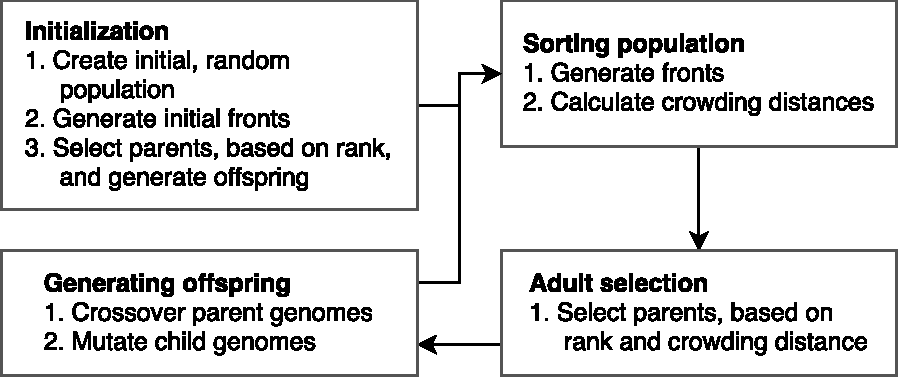
\includegraphics[scale=0.7]{overview.pdf}
    \caption{Flow of MOEA algorithm}
    \label{fig:overview}
\end{figure}

\subsubsection{Genotype}
The genotypes are represented as lists of all the city indices (zero-indexed), in the order that the salesman are visiting them. Different permutations of the list imply different routes for the salesman.

\subsubsection{Crossover}
For crossover, I used a customized version of the "ordered crossover" method.

The method creates a random number of intervals along the genome space. Even numbered intervals are copied from parent one to child one. Odd numbered intervals are copied from parent two to child two. The cities missing from each child is added in the order they appear in the opposite parent's genome.

Figure \ref{fig:crossover} shows an example of how the crossover method works.

By copying parts of the parents directly into the children, and then adding the missing cities, the crossover method ensures that all cities are part of the genome, and only once. The crossover method does therefore not yield infeasible offspring.

\begin{figure}
\end{figure}

\subsubsection{Mutation}
For mutation, I used the "reverse sequence mutation (RMS)" method.

When using RMS, a random interval along the genome is chosen. The gene order in the interval is reversed.

Figure \ref{fig:mutation} shows an example of how the mutation method works.

By reversing a subset of the original genome, the mutation method ensures that all cities are part of the genome, and only once. The mutation method does therefore not yield infeasible offspring.

\begin{figure}[H]
    \centering
    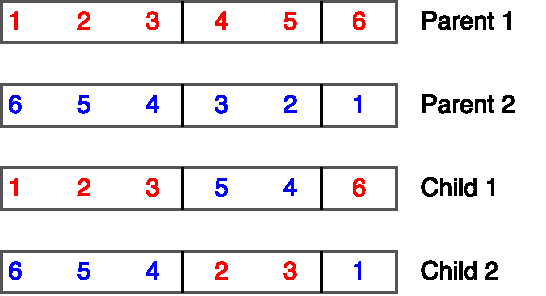
\includegraphics[width=.5\linewidth]{crossover.pdf}
    \caption{Visualisation of the crossover method}
    \label{fig:crossover}
\end{figure}
\begin{figure}[H]
    \centering
    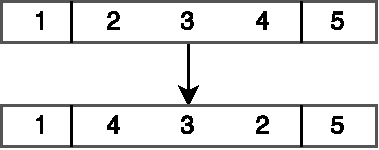
\includegraphics[width=.5\linewidth]{mutation.pdf}
    \caption{Visualisation of the mutation method}
    \label{fig:mutation}
\end{figure}


\section{Parameters}
\begin{tabulary}{\textwidth}{|L|L|L|L|L|L|L|L|L|}
    \hline
    \# & Population & Generations & Crossover rate & Mutation rate & Distance & Cost & Pareto-front size \\\hline
    1 & 300 & 200 & 0.5 & 0.5 & Max: 2199, min: 384 & Max: 192349, min: 66404 & 300 \\\hline
    2 & 100 & 500 & 0.5 & 0.5 & Max: 2098, min: 294 & Max: 180182, min: 86355 & 100 \\\hline
    3 & 200 & 500 & 0.9 & 0.5 & Max: 2255, min: 351 & Max: 183000, min: 72406 & 200 \\\hline
\end{tabulary}

\section{Results}

\begin{figure}[H]
    \centering
    \begin{subfigure}[b]{0.45\textwidth}
        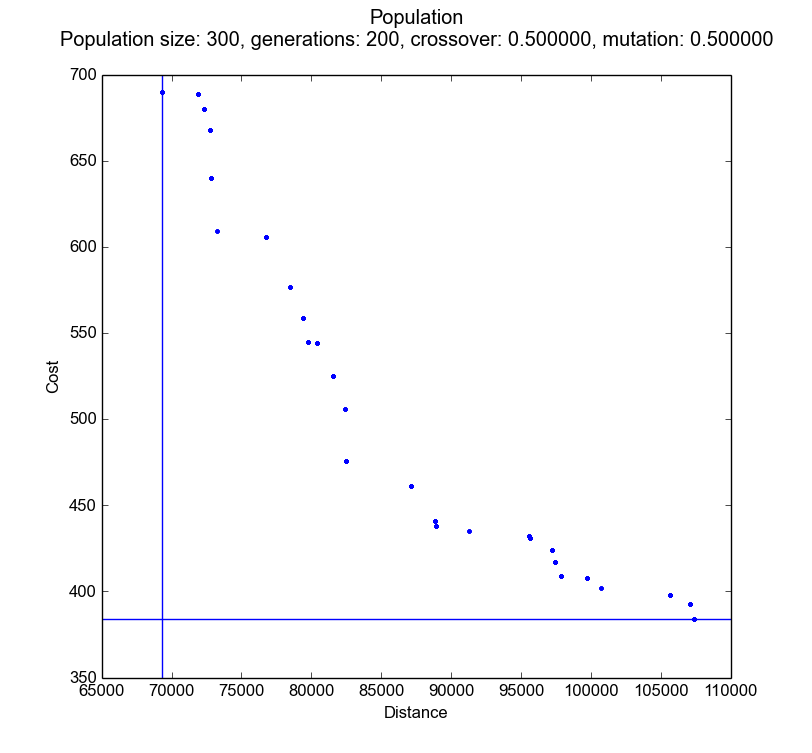
\includegraphics[width=\textwidth]{config-1-population.png}
        \caption{Population of configuration 1}
    \end{subfigure}
    \begin{subfigure}[b]{0.45\textwidth}
        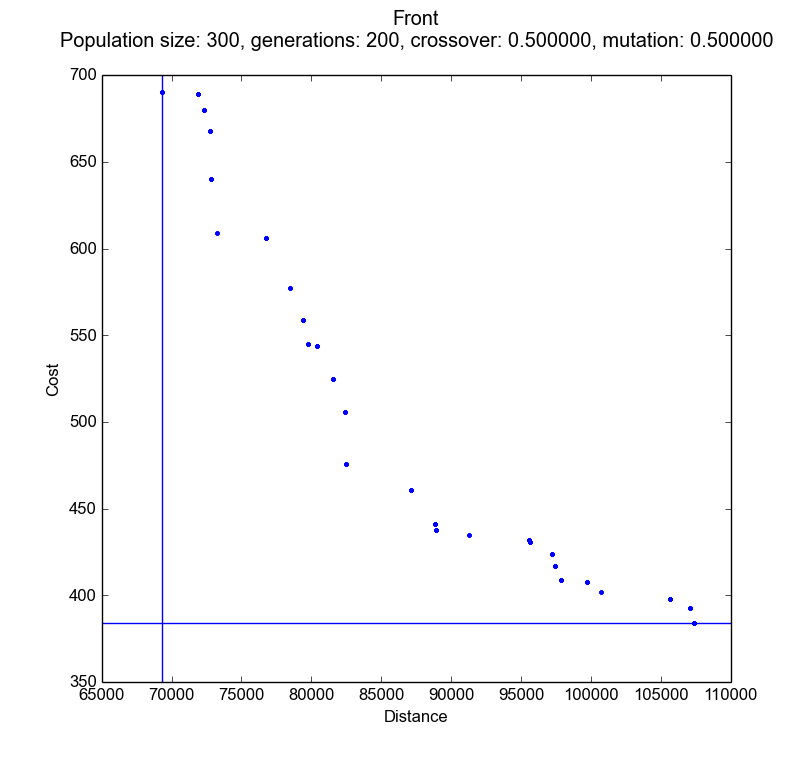
\includegraphics[width=\textwidth]{config-1-front.png}
        \caption{Pareto-front of configuration 1}
    \end{subfigure}
    \caption{Results for configuration 1}
    \label{config-1}
\end{figure}

\begin{figure}[H]
    \centering
    \begin{subfigure}[b]{0.45\textwidth}
        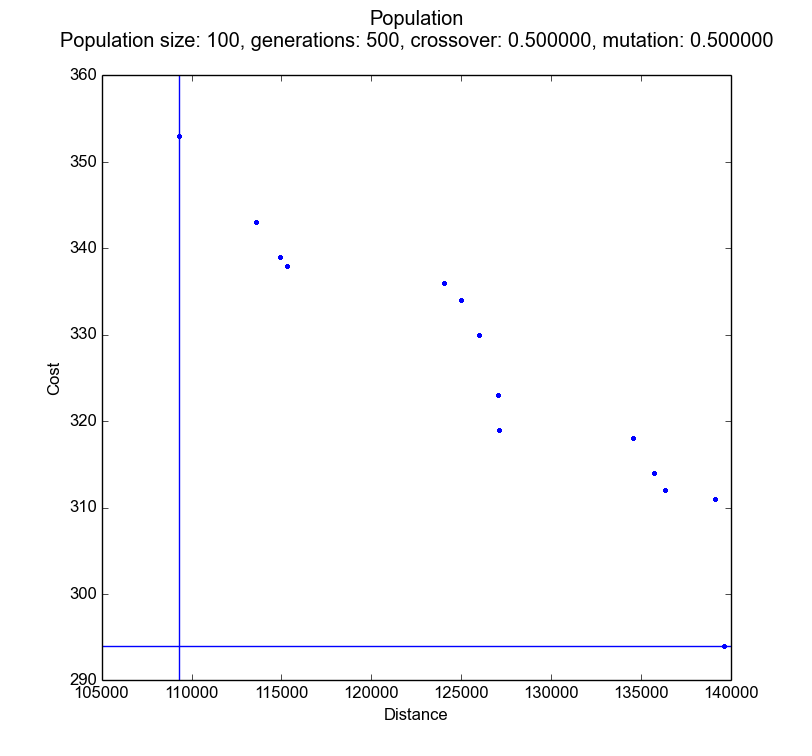
\includegraphics[width=\textwidth]{config-2-population.png}
        \caption{Population of configuration 2}
    \end{subfigure}
    \begin{subfigure}[b]{0.45\textwidth}
        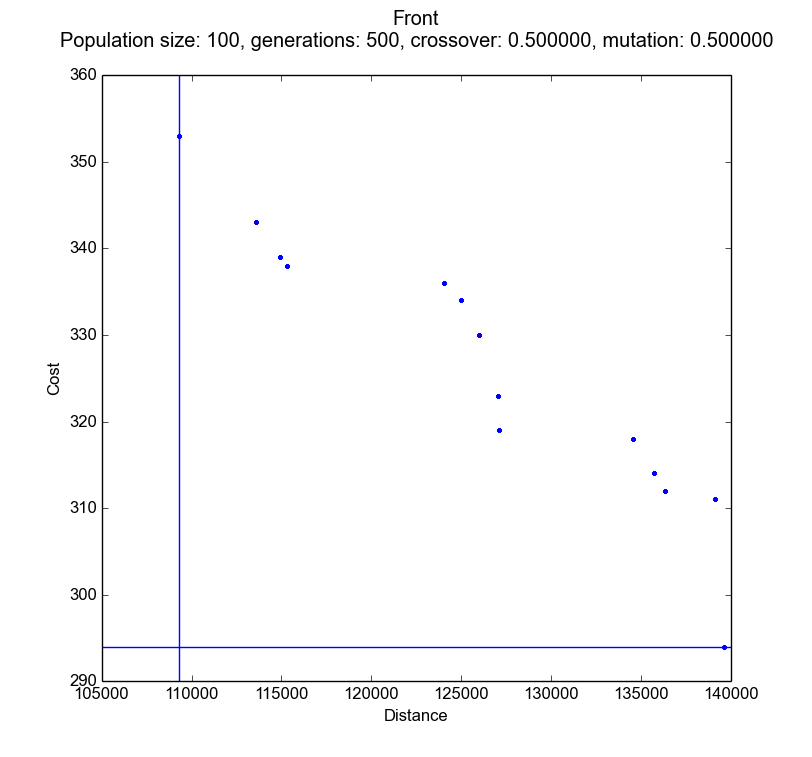
\includegraphics[width=\textwidth]{config-2-front.png}
        \caption{Pareto-front of configuration 2}
    \end{subfigure}
    \caption{Results for configuration 2}
    \label{config-2}
\end{figure}

\begin{figure}[H]
    \centering
    \begin{subfigure}[b]{0.45\textwidth}
        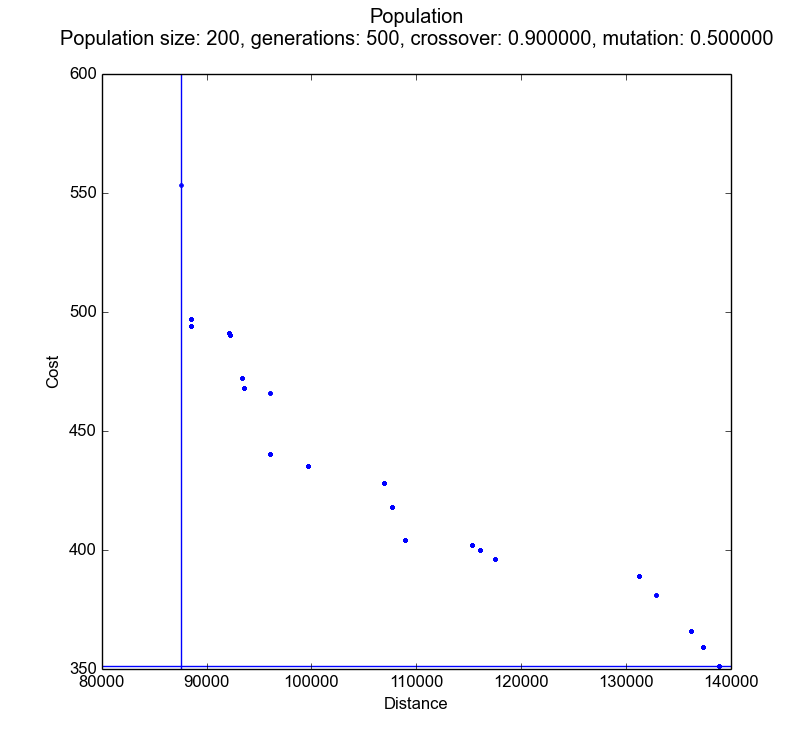
\includegraphics[width=\textwidth]{config-3-population.png}
        \caption{Population of configuration 3}
    \end{subfigure}
    \begin{subfigure}[b]{0.45\textwidth}
        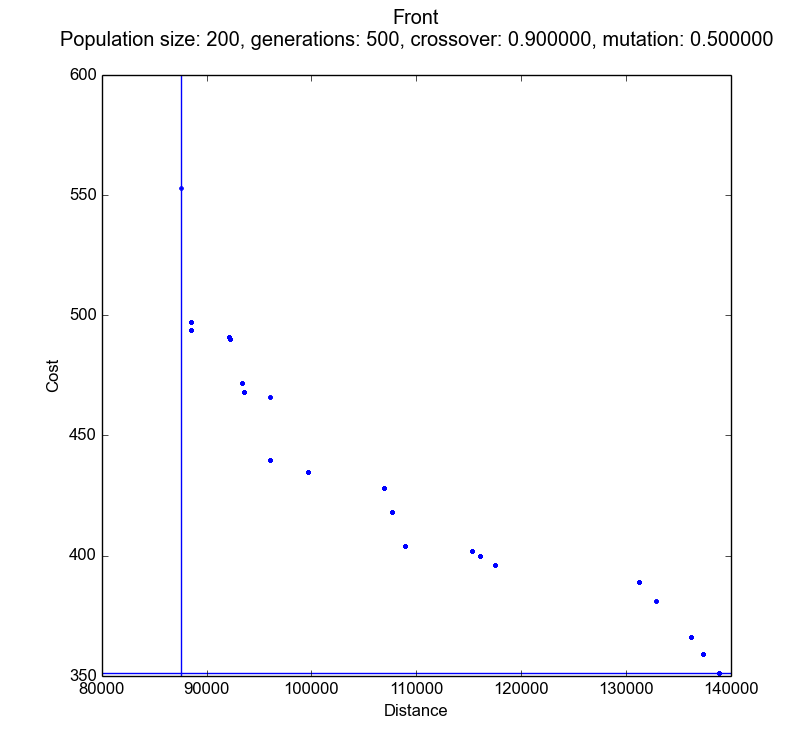
\includegraphics[width=\textwidth]{config-3-front.png}
        \caption{Pareto-front of configuration 3}
    \end{subfigure}
    \caption{Results for configuration 3}
    \label{config-3}
\end{figure}

As can be seen in Figures \ref{config-1}, \ref{config-2}, and \ref{config-3}, the final population converges towards the pareto front. This happens when the simulation is run for a certain amount of generations. The population is initially spread, but converges towards the front, as these solutions are among the best the algorithm can find with given configurations.

\begin{figure}[H]
    \centering
    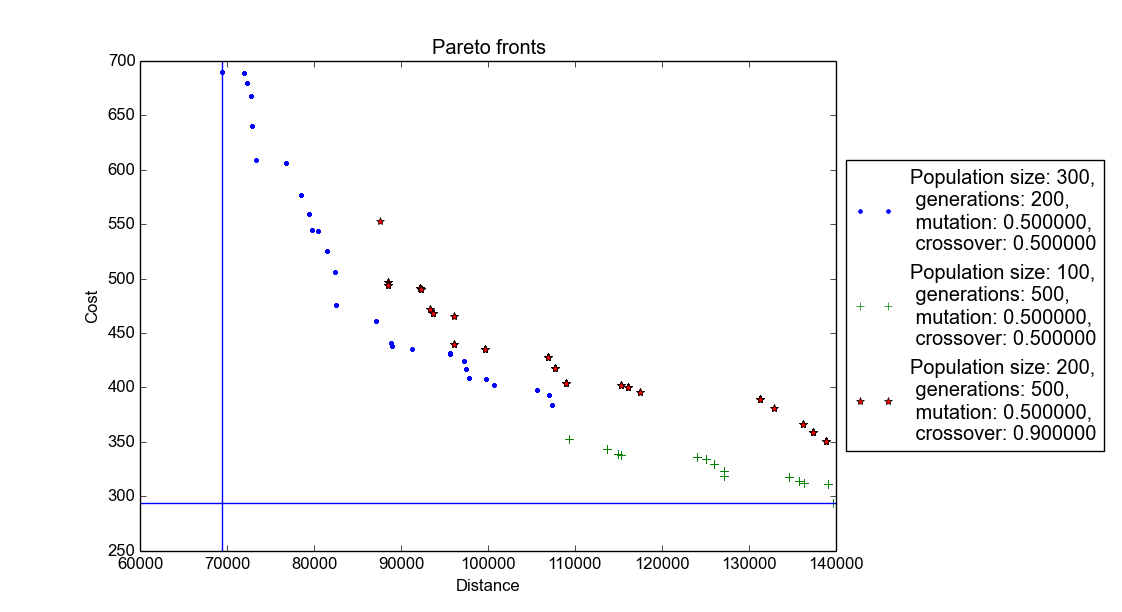
\includegraphics[scale=0.5]{all-configs-pareto.png}
    \caption{Comparison of the pareto-fronts of the different configurations}
\end{figure}

% End content

\end{document}
